\chapter{Swaption and Monte Carlo Simulation}    

In this chapter we'll start writing a class which represents an interest rate swap
(IRS) on a LIBOR index. The class will have a method which, given a
discount curve and a forward rate curve, will calculate the NPV of the
swap.
% (the latter curve will be used for determining the forward rates
%to calculate the expected value of the floating leg cash flows,
%whereas the former curve will be used to discount both the floating
%and fixed leg cash flows).

Next we will introduce interest rate swaptions and will write a similar class to 
handle them with methods for calculating the NPV analytically using the
Black-Scholes formula or via a Monte Carlo simulation.

\section{Interest Rate Swaps and Swaptions}\label{interest-rate-swaps-and-swaptions---lesson-6}

\subsection{EONIA vs EURIBOR}\label{eonia-vs-euribor}

Let's start by reminding ourselves of the differences and similarities
between the EONIA/OIS and EURIBOR/LIBOR interest rate markets.

\begin{itemize}
\tightlist
\item
  Similarities:

  \begin{itemize}
  \tightlist
  \item
    both are \textbf{unsecured} lending, i.e.~the lender assumes the
    risk of losing the capital if the borrower fails during the lending
    period;
  \item
    both represent some kind of \emph{average} interest rate between
    similar, large financial institutions.
  \end{itemize}
\end{itemize}

    \begin{itemize}
\tightlist
\item
  Differences:

  \begin{itemize}
  \tightlist
  \item
    EONIA/OIS:

    \begin{itemize}
    \tightlist
    \item
      are related to overnight lending, which needs to be renewed each
      day. This means that each day the lender can choose to not renew
      the loan or lend the capital to a different borrower;
    \item
      rates are a volume-weighted average of real transactions.
    \end{itemize}
  \item
    EURIBOR/LIBOR:

    \begin{itemize}
    \tightlist
    \item
      refer to term lending, i.e.~lending periods such as one month,
      three months, etc. The lender needs to wait until the expiration
      of the loan before having the option to lend the capital to a
      different borrower;
    \item
      are determined through a survey of panel banks' percieved market
      rates.
    \end{itemize}
  \end{itemize}
\end{itemize}

    A naive understanding of the interest rate markets would lead one to
believe that these different markets (O/N, 1M, 3M, etc) can all be
priced with a single discount curve - indeed in periods of low market
stress, this has been the case.

In reality, the details of the liquidity and counter-party risk involved
in each type of transaction are such that there is a basis between these
markets, and therefore each one has a different discount (or rate) curve
associated with it.

    Given the fact that LIBOR curves do not represent a \emph{pure} interest
rate market but incorporate elements of liquidity and counter-party risk,
it is surprising that, so many years after the financial crisis, they
still maintain so much importance as benchmark rate markets for a wide
range of purposes.

Indeed, though OIS markets are fully liquid enough to extract
information about forward interest rates, there is no functioning
options market from which to extract information about the volatility of
those interest rates. The liquidity in rate volatility continues to be
present only in the LIBOR swaptions markets.

As such, it continues to be important for banks to be able to price and
calibrate market parameters against LIBOR instruments.

\section{Interest Rate Swaps}\label{interest-rate-swaps}

Interest rate swaps consist of a floating leg and a fixed leg. The
contract parameters are:

\begin{itemize}
\tightlist
\item
  start date \(d_0\)
\item
  notional \(N\)
\item
  fixed rate \(K\)
\item
  floating rate tenor (months)
\item
  maturity (years)
\end{itemize}

The floating leg pays the reference LIBOR fixing at a frequency equal to
the tenor of the floating rate - so for example an IRS on a 3-month
LIBOR will pay a floating coupon every three months, an IRS on 6-month
EURIBOR pays the floating coupon every six months and so on.

The fixed leg pays a predetermined cash flow at annual frequency,
regardless of the tenor of the underlying floating rate. For simplicity
we will only consider swaps with maturities which are multiples of 1
year.

To make it even more useful, modify the \texttt{generate\_swap\_dates} function in
\texttt{finmarket} module to generate the payment dates for both the fixed
and floating legs, as follows:

    \begin{tcolorbox}[breakable, size=fbox, boxrule=1pt, pad at break*=1mm,colback=cellbackground, colframe=cellborder]
\begin{Verbatim}[commandchars=\\\{\}]
\PY{k+kn}{from} \PY{n+nn}{datetime} \PY{k}{import} \PY{n}{date}
\PY{k+kn}{from} \PY{n+nn}{dateutil}\PY{n+nn}{.}\PY{n+nn}{relativedelta} \PY{k}{import} \PY{n}{relativedelta}

\PY{k}{def} \PY{n+nf}{generate\PYZus{}swap\PYZus{}dates}\PY{p}{(}\PY{n}{start\PYZus{}date}\PY{p}{,} \PY{n}{n\PYZus{}months}\PY{p}{,} \PY{n}{tenor\PYZus{}months}\PY{o}{=}\PY{l+m+mi}{12}\PY{p}{)}\PY{p}{:}
    \PY{n}{dates} \PY{o}{=} \PY{p}{[}\PY{p}{]}
    \PY{k}{for} \PY{n}{n} \PY{o+ow}{in} \PY{n+nb}{range}\PY{p}{(}\PY{l+m+mi}{0}\PY{p}{,} \PY{n}{n\PYZus{}months}\PY{p}{,} \PY{n}{tenor\PYZus{}months}\PY{p}{)}\PY{p}{:}
        \PY{n}{dates}\PY{o}{.}\PY{n}{append}\PY{p}{(}\PY{n}{start\PYZus{}date} \PY{o}{+} \PY{n}{relativedelta}\PY{p}{(}\PY{n}{months}\PY{o}{=}\PY{n}{n}\PY{p}{)}\PY{p}{)}
    \PY{n}{dates}\PY{o}{.}\PY{n}{append}\PY{p}{(}\PY{n}{start\PYZus{}date} \PY{o}{+} \PY{n}{relativedelta}\PY{p}{(}\PY{n}{months}\PY{o}{=}\PY{n}{n\PYZus{}months}\PY{p}{)}\PY{p}{)}
    \PY{k}{return} \PY{n}{dates}

\PY{n}{generate\PYZus{}swap\PYZus{}dates}\PY{p}{(}\PY{n}{date}\PY{o}{.}\PY{n}{today}\PY{p}{(}\PY{p}{)}\PY{p}{,} \PY{l+m+mi}{16}\PY{p}{,} \PY{l+m+mi}{3}\PY{p}{)}

[datetime.date(2019, 10, 30),
 datetime.date(2020, 1, 30),
 datetime.date(2020, 4, 30),
 datetime.date(2020, 7, 30),
 datetime.date(2020, 10, 30),
 datetime.date(2021, 1, 30),
 datetime.date(2021, 2, 28)]
\end{Verbatim}
\end{tcolorbox}
        
    Using this function and the contract parameters we can determine a
sequence of payment dates for each of the two legs.

    Let \(d_0=d_0^{\mathrm{fixed}},...,d_p^{\mathrm{fixed}}\) be the fixed
leg payment dates and
\(d_0=d_0^{\mathrm{float}},...,d_p^{\mathrm{float}}\) be the floating
leg payment dates, and let's use the following notation:

\begin{itemize}
\tightlist
\item
  \(d\) the pricing date
\item
  \(D(d, d')\) the discount factor observed in date \(d\) for the value
  date \(d'\)
\item
  \(F(d, d', d'')\) the forward rate observed in date \(d\) for the
  period \([d', d'']\). The rate tenor is \(\tau = d'' - d'\).
\end{itemize}

    The NPV of the fixed leg is calculated as follows:

\[\mathrm{NPV}_{\mathrm{fixed}}(d; K) = N\cdot K\cdot\sum_{i=1}^{p}D(d, d_{i}^{\mathrm{fixed}})\]

and the NPV of the floating leg results:

\[\mathrm{NPV}_{\mathrm{float}}(d) = N\cdot\sum_{i=1}^{q}F(d, d_{j-1}^{\mathrm{float}}, d_{j}^{\mathrm{float}}) \cdot \frac{d_{j}^{\mathrm{float}}-d_{j-1}^{\mathrm{float}}}{360}
\cdot D(d, d_{i}^{\mathrm{float}})\]

Therefore the total NPV of the swap (seen from the point of view of the
counter-party which receives the floating leg) is:

\[\mathrm{NPV}(d; K) = \mathrm{NPV}_{\mathrm{float}}(d) - \mathrm{NPV}_{\mathrm{fixed}}(d;K)\]

    For reasons which will become apparent later, it's actually more
convenient to express the NPV of an IRS as a function of the fair value
fixed rate \(S\) of the IRS, also known as the \textbf{swap rate}. \(S\)
is the value of K which makes \(\mathrm{NPV}(d)=0\).

On the basis of the previous expressions, we can easily calculate \(S\) as:

\[\mathrm{NPV}_{\mathrm{fixed}}(d;S) = \mathrm{NPV}_{\mathrm{float}}(d)\]
\[N\cdot S\cdot\sum_{i=1}^{p}D(d, d_{i}^{\mathrm{fixed}}) = N\cdot\sum_{i=1}^{q}F(d, d_{j-1}^{\mathrm{float}}, d_{j}^{\mathrm{float}}) \cdot \frac{d_{j}^{\mathrm{float}}-d_{j-1}^{\mathrm{float}}}{360} \cdot D(d, d_{i}^{\mathrm{float}})\]
\[S=\frac{\sum_{i=1}^{q}F(d, d_{j-1}^{\mathrm{float}}, d_{j}^{\mathrm{float}}) \cdot \frac{d_{j}^{\mathrm{float}}-d_{j-1}^{\mathrm{float}}}{360}
\cdot D(d, d_{i}^{\mathrm{float}})}{\sum_{i=1}^{p}D(d, d_i^{\mathrm{fixed}})} \]

    Once we have calculated \(S\), we can express the \(\mathrm{NPV}\) of an
IRS as follows:

\begin{align*}\mathrm{NPV}(d; K) & = \mathrm{NPV}_{\mathrm{float}}(d) - \mathrm{NPV}_{\mathrm{fixed}}(d; K) = & \\ \\ &= \underbrace{\mathrm{NPV}_{\mathrm{float}}(d) - \mathrm{NPV}_{\mathrm{fixed}}(d; S)}_{\mathrm{=\;0}} + \mathrm{NPV}_{\mathrm{fixed}}(d;S) - \mathrm{NPV}_{\mathrm{fixed}}(d;K) & \\ & = N\cdot(S-K)\cdot\underbrace{\sum_{i=1}^{p}D(d, d_{i}^{\mathrm{fixed}})}_{\mathrm{'annuity'}}\end{align*}

    For convenience the relevant inputs that will be used later (observation
date, discount and libor curve definitions) have been saved in two files 
\(\href{https://repl.it/@MatteoSani/support6}{\textrm{discount\_curve.xlsx}}\)
and \(\href{https://repl.it/@MatteoSani/support6}{\textrm{libor\_curve.xlsx}}\).

\begin{tcolorbox}[breakable, size=fbox, boxrule=1pt, pad at break*=1mm,colback=cellbackground, colframe=cellborder]
\begin{Verbatim}[commandchars=\\\{\}]
\PY{k+kn}{from} \PY{n+nn}{datetime} \PY{k}{import} \PY{n}{date}
\PY{k+kn}{from} \PY{n+nn}{curve\PYZus{}data} \PY{k}{import} \PY{n}{pricing\PYZus{}date}\PY{p}{,} \PY{n}{discount\PYZus{}curve}\PY{p}{,} \PY{n}{libor\PYZus{}curve}
\PY{n+nb}{print}\PY{p}{(}\PY{n}{discount\PYZus{}curve}\PY{o}{.}\PY{n}{df}\PY{p}{(}\PY{n}{date}\PY{p}{(}\PY{l+m+mi}{2020}\PY{p}{,} \PY{l+m+mi}{1}\PY{p}{,} \PY{l+m+mi}{1}\PY{p}{)}\PY{p}{)}\PY{p}{)}
\PY{n+nb}{print} \PY{p}{(}\PY{n}{libor\PYZus{}curve}\PY{o}{.}\PY{n}{forward\PYZus{}rate}\PY{p}{(}\PY{n}{date}\PY{p}{(}\PY{l+m+mi}{2020}\PY{p}{,} \PY{l+m+mi}{1}\PY{p}{,} \PY{l+m+mi}{1}\PY{p}{)}\PY{p}{)}\PY{p}{)}

1.0003778376026289
0.01000266393442623
\end{Verbatim}
\end{tcolorbox}

    \begin{tcolorbox}[breakable, size=fbox, boxrule=1pt, pad at break*=1mm,colback=cellbackground, colframe=cellborder]
\begin{Verbatim}[commandchars=\\\{\}]
\PY{k+kn}{from} \PY{n+nn}{finmarkets} \PY{k}{import} \PY{n}{generate\PYZus{}swap\PYZus{}dates}

\PY{k}{class} \PY{n+nc}{InterestRateSwap}\PY{p}{:}
    
    \PY{k}{def} \PY{n+nf}{\PYZus{}\PYZus{}init\PYZus{}\PYZus{}}\PY{p}{(}\PY{n+nb+bp}{self}\PY{p}{,} \PY{n}{start\PYZus{}date}\PY{p}{,} \PY{n}{notional}\PY{p}{,} \PY{n}{fixed\PYZus{}rate}\PY{p}{,} \PY{n}{tenor\PYZus{}months}\PY{p}{,} 
                 \PY{n}{maturity\PYZus{}years}\PY{p}{)}\PY{p}{:}
        \PY{n+nb+bp}{self}\PY{o}{.}\PY{n}{notional} \PY{o}{=} \PY{n}{notional}
        \PY{n+nb+bp}{self}\PY{o}{.}\PY{n}{fixed\PYZus{}rate} \PY{o}{=} \PY{n}{fixed\PYZus{}rate}
        \PY{n+nb+bp}{self}\PY{o}{.}\PY{n}{fixed\PYZus{}leg\PYZus{}dates} \PY{o}{=} \PYZbs{}
            \PY{n}{generate\PYZus{}swap\PYZus{}dates}\PY{p}{(}\PY{n}{start\PYZus{}date}\PY{p}{,} \PY{l+m+mi}{12} \PY{o}{*} \PY{n}{maturity\PYZus{}years}\PY{p}{)}
        \PY{n+nb+bp}{self}\PY{o}{.}\PY{n}{floating\PYZus{}leg\PYZus{}dates} \PY{o}{=} \PYZbs{}
            \PY{n}{generate\PYZus{}swap\PYZus{}dates}\PY{p}{(}\PY{n}{start\PYZus{}date}\PY{p}{,} \PY{l+m+mi}{12} \PY{o}{*} \PY{n}{maturity\PYZus{}years}\PY{p}{,}
                                                      \PY{n}{tenor\PYZus{}months}\PY{p}{)}
        
    \PY{k}{def} \PY{n+nf}{annuity}\PY{p}{(}\PY{n+nb+bp}{self}\PY{p}{,} \PY{n}{discount\PYZus{}curve}\PY{p}{)}\PY{p}{:}
        \PY{n}{a} \PY{o}{=} \PY{l+m+mi}{0}
        \PY{k}{for} \PY{n}{i} \PY{o+ow}{in} \PY{n+nb}{range}\PY{p}{(}\PY{l+m+mi}{1}\PY{p}{,} \PY{n+nb}{len}\PY{p}{(}\PY{n+nb+bp}{self}\PY{o}{.}\PY{n}{fixed\PYZus{}leg\PYZus{}dates}\PY{p}{)}\PY{p}{)}\PY{p}{:}
            \PY{n}{a} \PY{o}{+}\PY{o}{=} \PY{n}{discount\PYZus{}curve}\PY{o}{.}\PY{n}{df}\PY{p}{(}\PY{n+nb+bp}{self}\PY{o}{.}\PY{n}{fixed\PYZus{}leg\PYZus{}dates}\PY{p}{[}\PY{n}{i}\PY{p}{]}\PY{p}{)}
        \PY{k}{return} \PY{n}{a}

    \PY{k}{def} \PY{n+nf}{swap\PYZus{}rate}\PY{p}{(}\PY{n+nb+bp}{self}\PY{p}{,} \PY{n}{discount\PYZus{}curve}\PY{p}{,} \PY{n}{libor\PYZus{}curve}\PY{p}{)}\PY{p}{:}
        \PY{n}{s} \PY{o}{=} \PY{l+m+mi}{0}
        \PY{k}{for} \PY{n}{j} \PY{o+ow}{in} \PY{n+nb}{range}\PY{p}{(}\PY{l+m+mi}{1}\PY{p}{,} \PY{n+nb}{len}\PY{p}{(}\PY{n+nb+bp}{self}\PY{o}{.}\PY{n}{floating\PYZus{}leg\PYZus{}dates}\PY{p}{)}\PY{p}{)}\PY{p}{:}
            \PY{n}{F} \PY{o}{=} \PY{n}{libor\PYZus{}curve}\PY{o}{.}\PY{n}{forward\PYZus{}rate}\PY{p}{(}\PY{n+nb+bp}{self}\PY{o}{.}\PY{n}{floating\PYZus{}leg\PYZus{}dates}\PY{p}{[}\PY{n}{j}\PY{o}{\PYZhy{}}\PY{l+m+mi}{1}\PY{p}{]}\PY{p}{)}
            \PY{n}{tau} \PY{o}{=} \PY{p}{(}\PY{n+nb+bp}{self}\PY{o}{.}\PY{n}{floating\PYZus{}leg\PYZus{}dates}\PY{p}{[}\PY{n}{j}\PY{p}{]} \PY{o}{\PYZhy{}} \PYZbs{}
                   \PY{n+nb+bp}{self}\PY{o}{.}\PY{n}{floating\PYZus{}leg\PYZus{}dates}\PY{p}{[}\PY{n}{j}\PY{o}{\PYZhy{}}\PY{l+m+mi}{1}\PY{p}{]}\PY{p}{)}\PY{o}{.}\PY{n}{days} \PY{o}{/} \PY{l+m+mi}{360}
            \PY{n}{P} \PY{o}{=} \PY{n}{discount\PYZus{}curve}\PY{o}{.}\PY{n}{df}\PY{p}{(}\PY{n+nb+bp}{self}\PY{o}{.}\PY{n}{floating\PYZus{}leg\PYZus{}dates}\PY{p}{[}\PY{n}{j}\PY{p}{]}\PY{p}{)}
            \PY{n}{s} \PY{o}{+}\PY{o}{=} \PY{n}{F} \PY{o}{*} \PY{n}{tau} \PY{o}{*} \PY{n}{P}
        \PY{k}{return} \PY{n}{s} \PY{o}{/} \PY{n+nb+bp}{self}\PY{o}{.}\PY{n}{annuity}\PY{p}{(}\PY{n}{discount\PYZus{}curve}\PY{p}{)}
        
    \PY{k}{def} \PY{n+nf}{npv}\PY{p}{(}\PY{n+nb+bp}{self}\PY{p}{,} \PY{n}{discount\PYZus{}curve}\PY{p}{,} \PY{n}{libor\PYZus{}curve}\PY{p}{)}\PY{p}{:}
        \PY{n}{S} \PY{o}{=} \PY{n+nb+bp}{self}\PY{o}{.}\PY{n}{swap\PYZus{}rate}\PY{p}{(}\PY{n}{discount\PYZus{}curve}\PY{p}{,} \PY{n}{libor\PYZus{}curve}\PY{p}{)}
        \PY{n}{A} \PY{o}{=} \PY{n+nb+bp}{self}\PY{o}{.}\PY{n}{annuity}\PY{p}{(}\PY{n}{discount\PYZus{}curve}\PY{p}{)}
        \PY{k}{return} \PY{n+nb+bp}{self}\PY{o}{.}\PY{n}{notional} \PY{o}{*} \PY{p}{(}\PY{n}{S} \PY{o}{\PYZhy{}} \PY{n+nb+bp}{self}\PY{o}{.}\PY{n}{fixed\PYZus{}rate}\PY{p}{)} \PY{o}{*} \PY{n}{A}
\end{Verbatim}
\end{tcolorbox}

    \begin{tcolorbox}[breakable, size=fbox, boxrule=1pt, pad at break*=1mm,colback=cellbackground, colframe=cellborder]
\prompt{In}{incolor}{4}{\boxspacing}
\begin{Verbatim}[commandchars=\\\{\}]
\PY{k+kn}{from} \PY{n+nn}{datetime} \PY{k}{import} \PY{n}{date}

\PY{n}{pricing\PYZus{}date} \PY{o}{=} \PY{n}{date}\PY{p}{(}\PY{l+m+mi}{2019}\PY{p}{,} \PY{l+m+mi}{11}\PY{p}{,} \PY{l+m+mi}{23}\PY{p}{)}
\PY{n}{irs} \PY{o}{=} \PY{n}{InterestRateSwap}\PY{p}{(}\PY{n}{pricing\PYZus{}date}\PY{p}{,} \PY{l+m+mf}{1e6}\PY{p}{,} \PY{l+m+mf}{0.05}\PY{p}{,} \PY{l+m+mi}{6}\PY{p}{,} \PY{l+m+mi}{4}\PY{p}{)}
\PY{n+nb}{print} \PY{p}{(}\PY{l+s+s2}{\PYZdq{}}\PY{l+s+si}{\PYZob{}:.2f\PYZcb{}}\PY{l+s+s2}{ EUR}\PY{l+s+s2}{\PYZdq{}}\PY{o}{.}\PY{n}{format}\PY{p}{(}\PY{n}{irs}\PY{o}{.}\PY{n}{npv}\PY{p}{(}\PY{n}{discount\PYZus{}curve}\PY{p}{,} \PY{n}{libor\PYZus{}curve}\PY{p}{)}\PY{p}{)}\PY{p}{)}

-160130.58 EUR
    \end{Verbatim}
\end{tcolorbox}

 Can you guess what could be the swap rate given that the NPV
is negative ? (Remember that we are looking at this contracts from the
point of view of the receiver of the floating leg$\ldots{}$)
Given that the fixed rate of the contract was 5\% we expect the swap rate to be smaller in order to reduce the NPV of the fixed leg.

    \begin{tcolorbox}[breakable, size=fbox, boxrule=1pt, pad at break*=1mm,colback=cellbackground, colframe=cellborder]
\begin{Verbatim}[commandchars=\\\{\}]
\PY{n+nb}{print} \PY{p}{(}\PY{l+s+s2}{\PYZdq{}}\PY{l+s+si}{\PYZob{}:.2f\PYZcb{}}\PY{l+s+s2}{\PYZdq{}}\PY{o}{.}\PY{n}{format}\PY{p}{(}\PY{n}{irs}\PY{o}{.}\PY{n}{swap\PYZus{}rate}\PY{p}{(}\PY{n}{discount\PYZus{}curve}\PY{p}{,} \PY{n}{libor\PYZus{}curve}\PY{p}{)}\PY{p}{)}\PY{p}{)}

0.01
    \end{Verbatim}
\end{tcolorbox}

    \begin{tcolorbox}[breakable, size=fbox, boxrule=1pt, pad at break*=1mm,colback=cellbackground, colframe=cellborder]
\begin{Verbatim}[commandchars=\\\{\}]
\PY{n}{irs2} \PY{o}{=} \PY{n}{InterestRateSwap}\PY{p}{(}\PY{n}{pricing\PYZus{}date}\PY{p}{,} \PY{l+m+mf}{1e6}\PY{p}{,} \PY{l+m+mf}{0.0102542}\PY{p}{,} \PY{l+m+mi}{6}\PY{p}{,} \PY{l+m+mi}{4}\PY{p}{)}
\PY{n+nb}{print} \PY{p}{(}\PY{l+s+s2}{\PYZdq{}}\PY{l+s+si}{\PYZob{}:.2f\PYZcb{}}\PY{l+s+s2}{ EUR}\PY{l+s+s2}{\PYZdq{}}\PY{o}{.}\PY{n}{format}\PY{p}{(}\PY{n}{irs2}\PY{o}{.}\PY{n}{npv}\PY{p}{(}\PY{n}{discount\PYZus{}curve}\PY{p}{,} \PY{n}{libor\PYZus{}curve}\PY{p}{)}\PY{p}{)}\PY{p}{)}

0.23 EUR
    \end{Verbatim}
\end{tcolorbox}

\section{Interest Rate Swaptions}\label{interest-rate-swaptions}

Swaptions are the equivalent of European options for the interest rate
markets. They give the option holder the right but not the obligation,
at the exercise date \(d_{ex}\), to enter into an IRS at a
pre-determined fixed rate.

Clearly the option holder will only choose to do this if the NPV of the
underlying swap at \(d_{ex}\) is positive - looking at the expression
for the NPV of the IRS in terms of the swap rate \(S\) therefore, we can
see that the payoff of the swaption is

\[N\cdot \mathrm{max}(0, S(d_{\mathrm{ex}}) - K)\cdot\sum D(d_{\mathrm{ex}}, d_i^{\mathrm{fixed}})\]

We now evaluate the NPV of a swaption with two alternative approaches.

\subsection{Evaluation through Black-Scholes
formula}\label{evaluation-through-black-scholes-formula}

In this case, to evaluate the NPV of this payoff, we'll use a
generalisation of the Black-Scholes formula applied to swaptions (it will not be derived here):

\[\mathrm{NPV} = N\cdot A\cdot [S \mathcal{N}(d_+) - K\mathcal{N}(d_-)]\]

where

\[d_{\pm} = \frac{\mathrm{log}(\frac{S}{K}) \pm \frac{1}{2}\sigma^{2}T}{\sigma\sqrt{T}}\;\; (\sigma\;\textrm{is the volatility of the swap rate})\\\]
\[A =\sum_{i=1}^{p}D(d, d_{i}^{\mathrm{fixed}})\;\;(\mathrm{annuity})\]

    \begin{tcolorbox}[breakable, size=fbox, boxrule=1pt, pad at break*=1mm,colback=cellbackground, colframe=cellborder]
\begin{Verbatim}[commandchars=\\\{\}]
\PY{n}{sigma} \PY{o}{=} \PY{l+m+mf}{0.07}
\PY{n}{irs} \PY{o}{=} \PY{n}{InterestRateSwap}\PY{p}{(}\PY{n}{pricing\PYZus{}date}\PY{p}{,} \PY{l+m+mf}{1e6}\PY{p}{,} \PY{l+m+mf}{0.01}\PY{p}{,} \PY{l+m+mi}{6}\PY{p}{,} \PY{l+m+mi}{4}\PY{p}{)}

\PY{k+kn}{from} \PY{n+nn}{curve\PYZus{}data} \PY{k}{import} \PY{n}{pricing\PYZus{}date}\PY{p}{,} \PY{n}{discount\PYZus{}curve}\PY{p}{,} \PY{n}{libor\PYZus{}curve}\PY{p}{,} \PY{n}{start\PYZus{}date}
\PY{k+kn}{from} \PY{n+nn}{scipy}\PY{n+nn}{.}\PY{n+nn}{stats} \PY{k}{import} \PY{n}{norm} 
\PY{k+kn}{import} \PY{n+nn}{math}
\PY{k+kn}{from} \PY{n+nn}{dateutil}\PY{n+nn}{.}\PY{n+nn}{relativedelta} \PY{k}{import} \PY{n}{relativedelta}

\PY{n}{exercise\PYZus{}date} \PY{o}{=} \PY{n}{start\PYZus{}date} \PY{o}{+} \PY{n}{relativedelta}\PY{p}{(}\PY{n}{years}\PY{o}{=}\PY{l+m+mi}{4}\PY{p}{)}
\PY{n}{A} \PY{o}{=} \PY{n}{irs}\PY{o}{.}\PY{n}{annuity}\PY{p}{(}\PY{n}{discount\PYZus{}curve}\PY{p}{)}
\PY{n}{S} \PY{o}{=} \PY{n}{irs}\PY{o}{.}\PY{n}{swap\PYZus{}rate}\PY{p}{(}\PY{n}{discount\PYZus{}curve}\PY{p}{,} \PY{n}{libor\PYZus{}curve}\PY{p}{)}
\PY{n}{T} \PY{o}{=} \PY{p}{(}\PY{n}{exercise\PYZus{}date} \PY{o}{\PYZhy{}} \PY{n}{pricing\PYZus{}date}\PY{p}{)}\PY{o}{.}\PY{n}{days} \PY{o}{/} \PY{l+m+mi}{365}
\PY{n}{d1} \PY{o}{=} \PY{p}{(}\PY{n}{math}\PY{o}{.}\PY{n}{log}\PY{p}{(}\PY{n}{S}\PY{o}{/}\PY{n}{irs}\PY{o}{.}\PY{n}{fixed\PYZus{}rate}\PY{p}{)} \PY{o}{+} \PY{l+m+mf}{0.5} \PY{o}{*} \PY{n}{sigma}\PY{o}{*}\PY{o}{*}\PY{l+m+mi}{2} \PY{o}{*} \PY{n}{T}\PY{p}{)} \PY{o}{/} \PY{p}{(}\PY{n}{sigma} \PY{o}{*} \PY{n}{T}\PY{o}{*}\PY{o}{*}\PY{l+m+mf}{0.5}\PY{p}{)}
\PY{n}{d2} \PY{o}{=} \PY{p}{(}\PY{n}{math}\PY{o}{.}\PY{n}{log}\PY{p}{(}\PY{n}{S}\PY{o}{/}\PY{n}{irs}\PY{o}{.}\PY{n}{fixed\PYZus{}rate}\PY{p}{)} \PY{o}{\PYZhy{}} \PY{l+m+mf}{0.5} \PY{o}{*} \PY{n}{sigma}\PY{o}{*}\PY{o}{*}\PY{l+m+mi}{2} \PY{o}{*} \PY{n}{T}\PY{p}{)} \PY{o}{/} \PY{p}{(}\PY{n}{sigma} \PY{o}{*} \PY{n}{T}\PY{o}{*}\PY{o}{*}\PY{l+m+mf}{0.5}\PY{p}{)}
\PY{n}{npv} \PY{o}{=} \PY{n}{irs}\PY{o}{.}\PY{n}{notional} \PY{o}{*} \PY{n}{A} \PY{o}{*} \PY{p}{(}\PY{n}{S} \PY{o}{*} \PY{n}{norm}\PY{o}{.}\PY{n}{cdf}\PY{p}{(}\PY{n}{d1}\PY{p}{)} \PY{o}{\PYZhy{}} \PY{n}{irs}\PY{o}{.}\PY{n}{fixed\PYZus{}rate} \PY{o}{*} \PY{n}{norm}\PY{o}{.}\PY{n}{cdf}\PY{p}{(}\PY{n}{d2}\PY{p}{)}\PY{p}{)}

\PY{n+nb}{print}\PY{p}{(}\PY{l+s+s2}{\PYZdq{}}\PY{l+s+s2}{Swaption NPV with BS: }\PY{l+s+si}{\PYZob{}:.3f\PYZcb{}}\PY{l+s+s2}{ EUR}\PY{l+s+s2}{\PYZdq{}}\PY{o}{.}\PY{n}{format}\PY{p}{(}\PY{n}{npv}\PY{p}{)}\PY{p}{)}

Swaption NPV with BS: 3330.741 EUR
    \end{Verbatim}
\end{tcolorbox}

So in this example using the Black-Scholes formula we find an NPV of the swaption at the exercise date of 

\subsection{Monte Carlo Simulation}\label{whats-monte-carlo-simulation}

The modern version of the Monte Carlo method was invented in the late
1940s by Stanislaw Ulam, while he was working on nuclear weapons
projects at the Los Alamos National Laboratory.
Monte Carlo methods, or Monte Carlo experiments, are a broad class of
computational algorithms that rely on repeated random sampling to obtain
numerical results. The underlying concept is to use randomness to solve
problems that might be deterministic in principle. Monte Carlo methods
are mainly used in three problem classes: optimisation, numerical
integration, and generating draws from a probability distribution.

In principle, Monte Carlo can be used to solve any problem
having a probabilistic interpretation since by the law of large numbers, the
expected value of some random variable can be approximated by taking the
empirical mean of independent samples of the variable.

    Monte Carlo methods vary, but tend to follow a particular pattern:

\begin{itemize}
\tightlist
\item
  define a domain of possible inputs;
\item
  generate inputs randomly from a probability distribution over the
  defined domain;
\item
  perform a deterministic computation on the generated inputs;
\item
  aggregate the results.
\end{itemize}

Monte Carlo simulation is widely used in many fields: engineering,
physics, computational biology, computer graphics, applied statistics,
artificial intelligence for games, search and rescue and of course
finance and business.

\subsubsection{Pseudo-Random Numbers}\label{pseudo-random-numbers}

Uses of Monte Carlo methods require large amounts of random numbers to
generate the inputs, and it was their use that spurred the development
of pseudorandom number generators. Every language has libraries that
allows to produce huge series of random numbers (with a periodicity of
\(2^{19937}\)). Those numbers are produced by algorithms that take as
input a \emph{seed} which determines univokely the series. This means
that setting the same seed you will produce the same set of numbers
every time (which is great for debugging purpouses).

In \texttt{python} the right module to use is \texttt{random} which has the
following useful functions:

\begin{itemize}
\tightlist
\item
  \texttt{seed} set the seed of the random number generator;
\item
  \texttt{random} returns a random number between 0 and 1 (with uniform
  probability);
\item
  \texttt{randint(min,\ max)} returns an integer random number between
  \texttt{min} and \texttt{max} (with uniform probability);
\item
  \texttt{sample(aList,\ k=n)} samples n elements from the list
  \texttt{aList}.
\end{itemize}

As usual for a more detailed description check \texttt{help(random)}.

    \begin{tcolorbox}[breakable, size=fbox, boxrule=1pt, pad at break*=1mm,colback=cellbackground, colframe=cellborder]
\begin{Verbatim}[commandchars=\\\{\}]
\PY{k+kn}{import} \PY{n+nn}{random} 

\PY{n}{random}\PY{o}{.}\PY{n}{seed}\PY{p}{(}\PY{l+m+mi}{1}\PY{p}{)}
\PY{n+nb}{print} \PY{p}{(}\PY{l+s+s2}{\PYZdq{}}\PY{l+s+s2}{seed is 1}\PY{l+s+s2}{\PYZdq{}}\PY{p}{)}
\PY{n+nb}{print}\PY{p}{(}\PY{n}{random}\PY{o}{.}\PY{n}{random}\PY{p}{(}\PY{p}{)}\PY{p}{)}
\PY{n+nb}{print}\PY{p}{(}\PY{n}{random}\PY{o}{.}\PY{n}{random}\PY{p}{(}\PY{p}{)}\PY{p}{)}

\PY{n}{random}\PY{o}{.}\PY{n}{seed}\PY{p}{(}\PY{l+m+mi}{2}\PY{p}{)}
\PY{n+nb}{print} \PY{p}{(}\PY{l+s+s2}{\PYZdq{}}\PY{l+s+s2}{seed is 2}\PY{l+s+s2}{\PYZdq{}}\PY{p}{)}
\PY{n+nb}{print}\PY{p}{(}\PY{n}{random}\PY{o}{.}\PY{n}{random}\PY{p}{(}\PY{p}{)}\PY{p}{)}
\PY{n+nb}{print}\PY{p}{(}\PY{n}{random}\PY{o}{.}\PY{n}{random}\PY{p}{(}\PY{p}{)}\PY{p}{)}

\PY{n}{random}\PY{o}{.}\PY{n}{seed}\PY{p}{(}\PY{l+m+mi}{1}\PY{p}{)}
\PY{n+nb}{print} \PY{p}{(}\PY{l+s+s2}{\PYZdq{}}\PY{l+s+s2}{seed is 1 again}\PY{l+s+s2}{\PYZdq{}}\PY{p}{)}
\PY{n+nb}{print}\PY{p}{(}\PY{n}{random}\PY{o}{.}\PY{n}{random}\PY{p}{(}\PY{p}{)}\PY{p}{)}
\PY{n+nb}{print}\PY{p}{(}\PY{n}{random}\PY{o}{.}\PY{n}{random}\PY{p}{(}\PY{p}{)}\PY{p}{)}

\PY{n+nb}{print}\PY{p}{(}\PY{n}{random}\PY{o}{.}\PY{n}{randint}\PY{p}{(}\PY{l+m+mi}{1}\PY{p}{,} \PY{l+m+mi}{10}\PY{p}{)}\PY{p}{)}
\PY{n}{aList} \PY{o}{=} \PY{p}{[}\PY{l+s+s1}{\PYZsq{}}\PY{l+s+s1}{a}\PY{l+s+s1}{\PYZsq{}}\PY{p}{,} \PY{l+s+s1}{\PYZsq{}}\PY{l+s+s1}{b}\PY{l+s+s1}{\PYZsq{}}\PY{p}{,} \PY{l+s+s1}{\PYZsq{}}\PY{l+s+s1}{c}\PY{l+s+s1}{\PYZsq{}}\PY{p}{,} \PY{l+s+s1}{\PYZsq{}}\PY{l+s+s1}{d}\PY{l+s+s1}{\PYZsq{}}\PY{p}{,} \PY{l+s+s1}{\PYZsq{}}\PY{l+s+s1}{f}\PY{l+s+s1}{\PYZsq{}}\PY{p}{]}
\PY{n+nb}{print} \PY{p}{(}\PY{n}{random}\PY{o}{.}\PY{n}{sample}\PY{p}{(}\PY{n}{aList}\PY{p}{,} \PY{n}{k}\PY{o}{=}\PY{l+m+mi}{2}\PY{p}{)}\PY{p}{)}

seed is 1
0.13436424411240122
0.8474337369372327
seed is 2
0.9560342718892494
0.9478274870593494
seed is 1 again
0.13436424411240122
0.8474337369372327
2
['c', 'a']
    \end{Verbatim}
\end{tcolorbox}

    \begin{tcolorbox}[breakable, size=fbox, boxrule=1pt, pad at break*=1mm,colback=cellbackground, colframe=cellborder]
\begin{Verbatim}[commandchars=\\\{\}]
\PY{n}{numbers} \PY{o}{=} \PY{p}{[}\PY{p}{]}
\PY{k}{for} \PY{n}{\PYZus{}} \PY{o+ow}{in} \PY{n+nb}{range}\PY{p}{(}\PY{l+m+mi}{10000}\PY{p}{)}\PY{p}{:}
  \PY{n}{numbers}\PY{o}{.}\PY{n}{append}\PY{p}{(}\PY{n}{random}\PY{o}{.}\PY{n}{randint}\PY{p}{(}\PY{l+m+mi}{0}\PY{p}{,} \PY{l+m+mi}{5}\PY{p}{)}\PY{p}{)}

\PY{k+kn}{from} \PY{n+nn}{matplotlib} \PY{k}{import} \PY{n}{pyplot} \PY{k}{as} \PY{n}{plt}
\PY{n}{plt}\PY{o}{.}\PY{n}{hist}\PY{p}{(}\PY{n}{numbers}\PY{p}{,} \PY{l+m+mi}{6}\PY{p}{,} \PY{n+nb}{range}\PY{o}{=}\PY{p}{[}\PY{o}{\PYZhy{}}\PY{l+m+mf}{0.5}\PY{p}{,} \PY{l+m+mf}{5.5}\PY{p}{]}\PY{p}{)}
\PY{n}{plt}\PY{o}{.}\PY{n}{title}\PY{p}{(}\PY{l+s+s2}{\PYZdq{}}\PY{l+s+s2}{Uniform distribution from randint}\PY{l+s+s2}{\PYZdq{}}\PY{p}{)}
\PY{n}{plt}\PY{o}{.}\PY{n}{show}\PY{p}{(}\PY{p}{)}
\end{Verbatim}
\end{tcolorbox}

    \begin{center}
    \adjustimage{max size={0.9\linewidth}{0.9\paperheight}}{lecture_6_files/lecture_6_28_0.png}
    \end{center}
    { \hspace*{\fill} \\}
    
\subsubsection{Practical Example of Monte Carlo
Simulation}\label{example-of-monte-carlo-simulation}

Let's check the probability to get two kings drawing randomly two cards
from a deck. Using a frequentist approach, we can calculate the
probability of an event as the ratio of the number of favourable outcomes
of an experiment (number of successes) and the number of all possible
outcomes so for our example:

\[P_\textrm{two kings} = \frac{4}{40} \cdot \frac{3}{39} = \frac{1}{130} \approx 0.0077\]

Let's now try with a Monte Carlo simulation.

    \begin{tcolorbox}[breakable, size=fbox, boxrule=1pt, pad at break*=1mm,colback=cellbackground, colframe=cellborder]
\begin{Verbatim}[commandchars=\\\{\}]
\PY{k+kn}{from} \PY{n+nn}{random} \PY{k}{import} \PY{n}{sample}\PY{p}{,} \PY{n}{choices}\PY{p}{,} \PY{n}{seed}

\PY{n}{seed}\PY{p}{(}\PY{l+m+mi}{1}\PY{p}{)}

\PY{n}{deck} \PY{o}{=} \PY{p}{[}\PY{l+s+s2}{\PYZdq{}}\PY{l+s+s2}{A}\PY{l+s+s2}{\PYZdq{}}\PY{p}{,} \PY{l+s+s2}{\PYZdq{}}\PY{l+s+s2}{2}\PY{l+s+s2}{\PYZdq{}}\PY{p}{,} \PY{l+s+s2}{\PYZdq{}}\PY{l+s+s2}{3}\PY{l+s+s2}{\PYZdq{}}\PY{p}{,} \PY{l+s+s2}{\PYZdq{}}\PY{l+s+s2}{4}\PY{l+s+s2}{\PYZdq{}}\PY{p}{,} \PY{l+s+s2}{\PYZdq{}}\PY{l+s+s2}{5}\PY{l+s+s2}{\PYZdq{}}\PY{p}{,} \PY{l+s+s2}{\PYZdq{}}\PY{l+s+s2}{6}\PY{l+s+s2}{\PYZdq{}}\PY{p}{,} \PY{l+s+s2}{\PYZdq{}}\PY{l+s+s2}{7}\PY{l+s+s2}{\PYZdq{}}\PY{p}{,} \PY{l+s+s2}{\PYZdq{}}\PY{l+s+s2}{J}\PY{l+s+s2}{\PYZdq{}}\PY{p}{,} \PY{l+s+s2}{\PYZdq{}}\PY{l+s+s2}{Q}\PY{l+s+s2}{\PYZdq{}}\PY{p}{,} \PY{l+s+s2}{\PYZdq{}}\PY{l+s+s2}{K}\PY{l+s+s2}{\PYZdq{}}\PY{p}{]} \PY{o}{*} \PY{l+m+mi}{4}

\PY{n}{trials} \PY{o}{=} \PY{l+m+mi}{1000000}
\PY{n}{success} \PY{o}{=} \PY{l+m+mi}{0}

\PY{k}{for} \PY{n}{i} \PY{o+ow}{in} \PY{n+nb}{range}\PY{p}{(}\PY{n}{trials}\PY{p}{)}\PY{p}{:}
  \PY{n}{cards} \PY{o}{=} \PY{n}{sample}\PY{p}{(}\PY{n}{deck}\PY{p}{,} \PY{n}{k}\PY{o}{=}\PY{l+m+mi}{2}\PY{p}{)}
  \PY{k}{if} \PY{n}{i} \PY{o}{\PYZlt{}} \PY{l+m+mi}{10}\PY{p}{:}
    \PY{n+nb}{print} \PY{p}{(}\PY{n}{cards}\PY{p}{)}
  \PY{k}{if} \PY{n}{cards} \PY{o}{==} \PY{p}{[}\PY{l+s+s2}{\PYZdq{}}\PY{l+s+s2}{K}\PY{l+s+s2}{\PYZdq{}}\PY{p}{,} \PY{l+s+s2}{\PYZdq{}}\PY{l+s+s2}{K}\PY{l+s+s2}{\PYZdq{}}\PY{p}{]}\PY{p}{:}
    \PY{n}{success} \PY{o}{+}\PY{o}{=} \PY{l+m+mi}{1}
    
\PY{n+nb}{print} \PY{p}{(}\PY{l+s+s2}{\PYZdq{}}\PY{l+s+s2}{The probability to draw two kings is }\PY{l+s+si}{\PYZob{}:.4f\PYZcb{}}\PY{l+s+s2}{\PYZdq{}}\PY{o}{.}\PY{n}{format}\PY{p}{(}\PY{n}{success}\PY{o}{/}\PY{n}{trials}\PY{p}{)}\PY{p}{)}

['Q', '7']
['5', '7']
['J', '2']
['Q', 'A']
['5', '4']
['7', '2']
['2', '5']
['J', 'Q']
['A', 'Q']
['J', '5']
The probability to draw two kings is 0.0077
    \end{Verbatim}
\end{tcolorbox}

    Other modules provide random generators according to different
distributions. Below an example with \texttt{numpy.random} which allows
to throw random numbers according to a normal distribution
(\(\mathcal{N}(0, 1)\)).

    \begin{tcolorbox}[breakable, size=fbox, boxrule=1pt, pad at break*=1mm,colback=cellbackground, colframe=cellborder]
\begin{Verbatim}[commandchars=\\\{\}]
\PY{k+kn}{from} \PY{n+nn}{numpy}\PY{n+nn}{.}\PY{n+nn}{random} \PY{k}{import} \PY{n}{normal}
\PY{k+kn}{from} \PY{n+nn}{matplotlib} \PY{k}{import} \PY{n}{pyplot} \PY{k}{as} \PY{n}{plt}

\PY{n}{gauss} \PY{o}{=} \PY{p}{[}\PY{p}{]}
\PY{k}{for} \PY{n}{\PYZus{}} \PY{o+ow}{in} \PY{n+nb}{range}\PY{p}{(}\PY{l+m+mi}{50000}\PY{p}{)}\PY{p}{:}
  \PY{n}{gauss}\PY{o}{.}\PY{n}{append}\PY{p}{(}\PY{n}{normal}\PY{p}{(}\PY{p}{)}\PY{p}{)}
  
\PY{n}{plt}\PY{o}{.}\PY{n}{hist}\PY{p}{(}\PY{n}{gauss}\PY{p}{,} \PY{l+m+mi}{100}\PY{p}{,} \PY{n+nb}{range}\PY{o}{=}\PY{p}{[}\PY{o}{\PYZhy{}}\PY{l+m+mi}{4}\PY{p}{,} \PY{l+m+mi}{4}\PY{p}{]}\PY{p}{)}
\PY{n}{plt}\PY{o}{.}\PY{n}{title}\PY{p}{(}\PY{l+s+s2}{\PYZdq{}}\PY{l+s+s2}{Example of gaussian distribution from numpy}\PY{l+s+s2}{\PYZdq{}}\PY{p}{)}
\PY{n}{plt}\PY{o}{.}\PY{n}{show}\PY{p}{(}\PY{p}{)}
\end{Verbatim}
\end{tcolorbox}

    \begin{center}
    \adjustimage{max size={0.9\linewidth}{0.9\paperheight}}{lecture_6_files/lecture_6_32_0.png}
    \end{center}
    { \hspace*{\fill} \\}
    
 \subsubsection{Derivation of log-normal Stochastic Differential
Equation}\label{derivation-of-log-normal-stochastic-differential-equation}

Stock prices deviate from a steady state as a result of the random
fluctuations given by the trades. Considering a stock with a price
\(S_t\) and an expected rate of return \(\mu\), then the relative change
in its price during a period \(dt\) can be decomposed in two parts:

\begin{itemize}
\tightlist
\item
  a deterministic part that is the expected return from the stock held
  during the time period \(dt\) (\(\mu S_tdt\))
\item
  a stochastic part which reflects the random changes of the market
  (e.g.~as a response to external effects such as unexpected news). A
  reasonable assumption is to take this contribution proportional to the
  stock (\(\sigma S_tdB_t\) where \(dB_t\) is a random walk process
  equal to \(\mathcal{N}(0,1)\sqrt{t}\)).
\end{itemize}

    The resulting differential equation is:

\[dS_t = \mu S_tdt + \sigma S_tdB_t\] or
\[\frac{dS_t}{S_t} = d\textrm{log}(S_t) = \mu dt + \sigma dB_t\]

    The solution of this equation can be derived by applying the
It\(\hat{o}\)'s formula which states that for any given function
\(G(S, t)\) where \(S\) satisfies the following stochastic differential
equation \(dS=a\cdot dt +b\cdot dB_t\) it holds:

\[dG=\big(a\frac{\partial G}{\partial S} + \frac{\partial G}{\partial t} + \frac{1}{2}b^2\frac{\partial^2 G}{\partial S^2} \big)dt + b \frac{\partial G}{\partial S}dB\]

Considering \(G = \textrm{log}(S_t)\) we have:

\[\frac{\partial G}{\partial S} = \frac{1}{S_t}\]

\[\frac{\partial G}{\partial t} = 0\]

\[\frac{\partial^2 G}{\partial S^2} = -\frac{1}{S_t^{2}}\]

    By inserting these into It\(\hat{o}\)'s formula we get:

\[d(\textrm{log} S_t) = \big(\mu S_t \frac{1}{S_t} + \frac{1}{2}\sigma^2 S_t^2 (-\frac{1}{S_t^2})\big)dt + \sigma\epsilon\sqrt{dt}\]

\[d(\textrm{log} S_t) = \textrm{log} (S_t) - \textrm{log} (S_{t-1}) = \textrm{log} \frac{S_t}{S_{t-1}} = \big(\mu - \frac{1}{2}\sigma^2\big)dt + \sigma\epsilon\sqrt{dt}\]

\[S_t = S_{t-1}e^{\big(\mu - \frac{1}{2}\sigma^2\big)dt + \sigma\epsilon\sqrt{dt}}\]

    As can be seen from the following equation:

\[d(\textrm{log} S_t) = \big(\mu - \frac{1}{2}\sigma^2\big)dt + \sigma\epsilon\sqrt{dt}\]
the change in \(\textrm{log} S_t\) has a constant \emph{drift}
\(\mu - \frac{1}{2}\sigma^2\) and a constance variance rate \(\sigma^2\)
(remember that \(\epsilon\) is a normally distributed random variable
(\(\mathcal{N}(0,1)\)). So you have a constant plus a gaussian
distributed variable, therefore \(\textrm{log} S_t\) at some time \(T\)
is normally distributed with:

\[\textrm{log}S_t - \textrm{log}S_0 \approx\mathcal{N}\big[\big(\mu-\frac{\sigma^2}{2}\big)T, \sigma^2 T\big]\]

This equation shows that \(\textrm{log}S_t\) is normally distributed,
but \textbf{a variable whose logarithm is normally distributed is said
to be log-normal}. Hence the model we have just developed implies that
the stock price at time T, given today's price, is lognormally
distributed. One of the nicer property of a log-normal distribution is to be positive defined 
and that's why lognormality is important because we need to ensure that a stock price
will never be negative. Indeed looking at the initial \(dS\) equation we
have that:

\[dS_t = \mu S_tdt + \sigma S_tdB_t\]
which shows that the closer is \(S_t\) to 0 the smaller is the \(dS\)
variation (so it will never go below 0).

\subsection{Evaluation through Monte-Carlo
Simulation}\label{evaluation-through-monte-carlo-simulation}

In this second case we start from the current swap rate \(S(d)\)
evaluated at the pricing date \(d\), and assume that it follows a
log-normal stochastic process, so its distribution at
\(d_{\mathrm{ex}}\) (exercise date) is
\(S(d_{\mathrm{ex}}) = S(d)\mathrm{exp}(-\frac{1}{2}\sigma^{2}T+\sigma\sqrt{T}\epsilon)\)
where \(\epsilon\approx\mathcal{N}(0,1)\). Remember that the discounted
payoff is given by:

\[N\cdot \mathrm{max}(0, S(d_{\mathrm{ex}}) - K)\cdot\sum D(d_{\mathrm{ex}}, d_i^{\mathrm{fixed}})\]

So to perform the simulation:

\begin{itemize}
\tightlist
\item
  we sample the normal distribution \(\mathcal{N}\) to calculate a large
  number of scenarios for \(S(d_{\mathrm{ex}})\);
\item
  we evaluate the underlying swap's NPV at the expiry date, and
  consequently the swaption's payoff, and finally take the average of these
  values to get its estimate.
\end{itemize}

    \begin{tcolorbox}[breakable, size=fbox, boxrule=1pt, pad at break*=1mm,colback=cellbackground, colframe=cellborder]
\begin{Verbatim}[commandchars=\\\{\}]
\PY{c+c1}{\PYZsh{} we\PYZsq{}ll need numpy.mean and numpy.std to calculate the average and standard }
\PY{c+c1}{\PYZsh{} deviation of a list of values}
\PY{k+kn}{import} \PY{n+nn}{numpy} \PY{k}{as} \PY{n+nn}{np}
\PY{k+kn}{from} \PY{n+nn}{numpy}\PY{n+nn}{.}\PY{n+nn}{random} \PY{k}{import} \PY{n}{normal}\PY{p}{,} \PY{n}{seed}

\PY{c+c1}{\PYZsh{} define the number of Monte Carlo scenarios}
\PY{n}{n\PYZus{}scenarios} \PY{o}{=} \PY{l+m+mi}{50000}
\PY{n}{discounted\PYZus{}payoffs} \PY{o}{=} \PY{p}{[}\PY{p}{]}
\PY{n}{seed}\PY{p}{(}\PY{l+m+mi}{1}\PY{p}{)}

\PY{k}{for} \PY{n}{i\PYZus{}scenario} \PY{o+ow}{in} \PY{n+nb}{range}\PY{p}{(}\PY{n}{n\PYZus{}scenarios}\PY{p}{)}\PY{p}{:}
    \PY{c+c1}{\PYZsh{} simulate the swap rate in this scenario}
    \PY{n}{S\PYZus{}simulated} \PY{o}{=} \PY{n}{S} \PY{o}{*} \PY{n}{math}\PY{o}{.}\PY{n}{exp}\PY{p}{(}\PY{o}{\PYZhy{}}\PY{l+m+mf}{0.5} \PY{o}{*} \PY{n}{sigma} \PY{o}{*} \PY{n}{sigma} \PY{o}{*} \PY{n}{T} \PY{o}{+}
                               \PY{n}{sigma} \PY{o}{*} \PY{n}{math}\PY{o}{.}\PY{n}{sqrt}\PY{p}{(}\PY{n}{T}\PY{p}{)} \PY{o}{*} \PY{n}{normal}\PY{p}{(}\PY{p}{)}\PY{p}{)}
    
    \PY{c+c1}{\PYZsh{} calculate the swap NPV in this scenario}
    \PY{n}{swap\PYZus{}npv} \PY{o}{=} \PY{n}{irs}\PY{o}{.}\PY{n}{notional} \PY{o}{*} \PY{p}{(}\PY{n}{S\PYZus{}simulated} \PY{o}{\PYZhy{}} \PY{n}{irs}\PY{o}{.}\PY{n}{fixed\PYZus{}rate}\PY{p}{)} \PY{o}{*} \PY{n}{A}
    
    \PY{c+c1}{\PYZsh{} add the discounted payoff of the swaption, in this scenario, to the list}
    \PY{n}{discounted\PYZus{}payoffs}\PY{o}{.}\PY{n}{append}\PY{p}{(}\PY{n+nb}{max}\PY{p}{(}\PY{l+m+mi}{0}\PY{p}{,} \PY{n}{swap\PYZus{}npv}\PY{p}{)}\PY{p}{)}
    
\PY{c+c1}{\PYZsh{} calculate the NPV of the swaption by taking the average of the discounted }
\PY{c+c1}{\PYZsh{} payoffs across all the scenarios}
\PY{n}{npv\PYZus{}mc} \PY{o}{=} \PY{n}{np}\PY{o}{.}\PY{n}{mean}\PY{p}{(}\PY{n}{discounted\PYZus{}payoffs}\PY{p}{)}
    
\PY{c+c1}{\PYZsh{} calculate the Monte Carlo error estimate for \PYZsq{}npv\PYZus{}mc\PYZsq{} this will give us a 99\PYZpc{} }
\PY{c+c1}{\PYZsh{} confidence interval for the calculated value (3 sigmas)}
\PY{n}{npv\PYZus{}error} \PY{o}{=} \PY{l+m+mi}{3} \PY{o}{*} \PY{n}{np}\PY{o}{.}\PY{n}{std}\PY{p}{(}\PY{n}{discounted\PYZus{}payoffs}\PY{p}{)} \PY{o}{/} \PY{n}{math}\PY{o}{.}\PY{n}{sqrt}\PY{p}{(}\PY{n}{n\PYZus{}scenarios}\PY{p}{)}

\PY{n+nb}{print}\PY{p}{(}\PY{l+s+s2}{\PYZdq{}}\PY{l+s+s2}{Swaption NPV: }\PY{l+s+si}{\PYZob{}:.2f\PYZcb{}}\PY{l+s+s2}{ EUR (+- }\PY{l+s+si}{\PYZob{}:.2f\PYZcb{}}\PY{l+s+s2}{ EUR with 99}\PY{l+s+si}{\PYZpc{} c}\PY{l+s+s2}{onfidence)}\PY{l+s+s2}{\PYZdq{}}\PYZbs{}
      \PY{o}{.}\PY{n}{format}\PY{p}{(}\PY{n}{npv\PYZus{}mc}\PY{p}{,} \PY{n}{npv\PYZus{}error}\PY{p}{)}\PY{p}{)}

Swaption NPV: 3351.42 EUR (+- 66.14 EUR with 99\% confidence)
    \end{Verbatim}
\end{tcolorbox}

Note that this is not \emph{strictly speaking} the correct way of calculating the value, the reason being that one should calculate the swap NPV at the expiry date of the swaption, apply the payoff function max(0, ...) and *then* discount from the expiry date to today.
However, it's simpler to calculate it as above and it doesn't make any difference to the result, since:

\[\textrm{DF * max(0, SwapNPVAtExpiry) == max(0, DF * SwapNPVAtExpiry)}\].

The NPV calculated via the Black-Scholes formula falls within the
confidence interval produced by the Monte Carlo simulation, so we can
assert that the two methods are in agreement.

\begin{itemize}
\tightlist
\item
  Swaption NPV (BS): 3330.74 EUR
\item
  Swaption NPV (MC): 3351.42 EUR
\end{itemize}

\subsection{Confidence interval}\label{confidence-interval}

X\% confidence interval can be interpreted by saying that there is X\%
probability that the calculated interval from another (different)
simulation contains the true value of the population parameter. In other
words X\% confidence interval can be expressed in terms of repeated
experiments (or samples): if you repeat many time the above simulation,
hence \(\mathcal{N}\) is sampled many times, the fraction of calculated
confidence intervals (which would differ for each sample) that contains
the true population parameter would tend toward X\%

\begin{figure}[h]
\centering
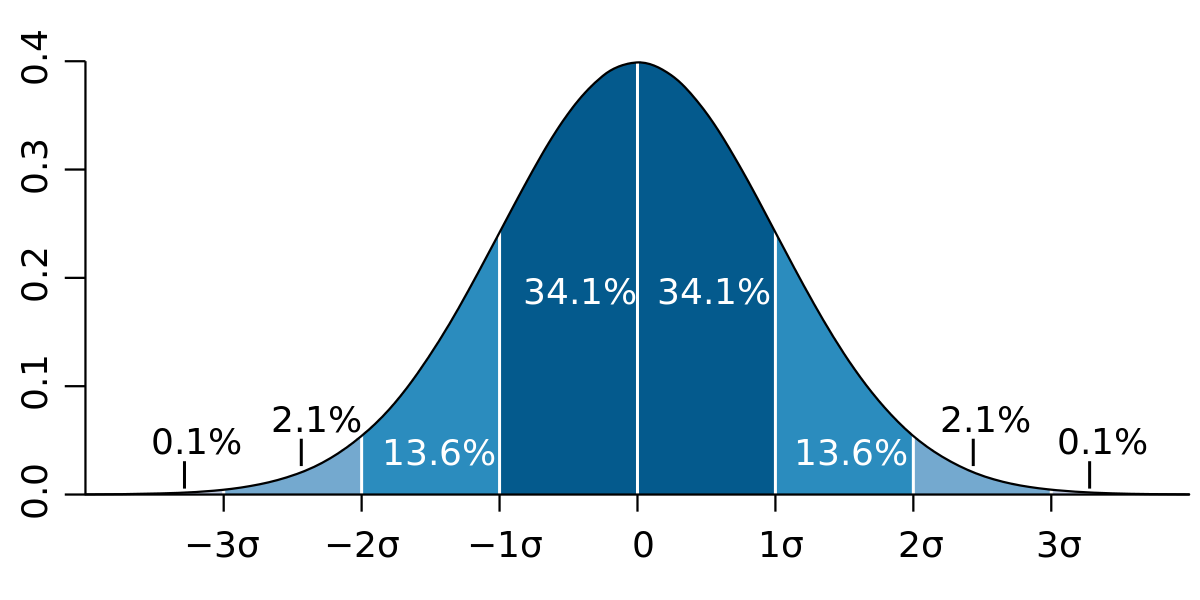
\includegraphics{Standard_deviation_diagram.svg.png}
\caption{Confidence interval graphical explanation}
\end{figure}

 